%\documentclass[jou]{apa6}
\documentclass[11pt]{article}
\usepackage{ucs}
\usepackage[utf8x]{inputenc}
\usepackage{changepage}
\usepackage{graphicx}
\usepackage{amsmath}
\usepackage{gensymb}
\usepackage{amssymb}
\usepackage{enumerate}
\usepackage{tabularx}
\usepackage{lipsum}
\usepackage{hyperref}
\usepackage{fancyvrb}

\oddsidemargin 0.0in
\evensidemargin 0.0in
\textwidth 6.27in
\headheight 1.0in
\topmargin -0.1in
\headheight 0.0in
\headsep 0.0in
\textheight 9.0in

\usepackage{xcolor}

\setlength\parindent{0pt}

\newenvironment{myenv}{\begin{adjustwidth}{0.4in}{0.4in}}{\end{adjustwidth}}
\renewcommand{\abstractname}{Anotācija}
\renewcommand\refname{Atsauces}



\newcounter{alphnum}
\newenvironment{alphlist}{\begin{list}{(\Alph{alphnum})}{\usecounter{alphnum}\setlength{\leftmargin}{2.5em}} \rm}{\end{list}}


%16.3-6

\makeatletter
\let\saved@bibitem\@bibitem
\makeatother

\usepackage{bibentry}
%\usepackage{hyperref}



\begin{document}
\thispagestyle{empty}

\twocolumn


\begin{center}
{\Large Assignment 1, 2020-09-14}
\end{center}


{\bf Question 1 (Bitwise Operations).} Write the output
(and the content of variables {\tt a,b,c} in hexadecimal notation),
after this snipped is executed:



\begin{center}
\begin{minipage}{.8\columnwidth}
\begin{Verbatim}[frame=single,numbers=left]
#include <iostream>
using namespace std;
int main() {
    unsigned int a = 
      0xACE02468;
    unsigned int b = 
      (a << 12) & (a >> 20);
    unsigned int c = 
      (a << 12) | (a >> 20);
    cout << hex << 
      "a = " << a << endl;
    cout << hex << 
      "b = " << b << endl;
    cout << hex << 
      "c = " << c << endl;
}
\end{Verbatim}
\end{minipage}
\end{center}

Hexadecimal memory content of variables:

% \rule{4cm}{0.4pt} 

\begin{tabular}{|c|c|} \hline
{\bf Variable} & {\bf Hex value} \\ \hline
{\tt \LARGE a} & \mbox{}\hspace{150pt}\mbox{} \\[20pt] \hline
{\tt \LARGE b} & \\[20pt] \hline
{\tt \LARGE c} & \\[20pt] \hline
\end{tabular}

{\em Note.} Unsigned ints are $4$ bytes long. 
If you do a right shift on 
such variables (by some $n$ bits), then the first $n$ bits 
on the left are filled with zeroes.









\vspace{20pt}
{\bf Question 2.} 
Draw a flowchart for this {\tt switch-case} statement.

\begin{center}
\begin{minipage}{.8\columnwidth}
\begin{Verbatim}[frame=single,numbers=left]
int x = 0;
char c; 
cin >> c; 
switch( c ) {
    case 'A':
        x += 1;
    case 'B':
        x += 2;
        break;
    default :
        x += 4;
}
cout << "x= " << x << endl;
\end{Verbatim}
\end{minipage}
\end{center}



Use only $5$ kinds of nodes:\\
{\footnotesize
{\bf (1)} Start node (oval: one outgoing arrow).\\
{\bf (2)} End node (oval: one incoming arrow).\\
{\bf (3)} Conditional statement (diamond: one incoming and two outgoing arrows). Mark the ``true'' branch.\\
{\bf (4)} Regular statement (rectangle: one incoming and one outgoing arrow).\\
{\bf (5)} Merging two branches (black dot: two incoming arrows, one outgoing arrow).
}



\vspace{20pt}
{\bf Question 3 (Side Effects).}
What is the value of {\tt x} output by the code snippet above, 
if {\tt cin} inputs letter {\tt 'A'}?


\newpage
{\bf \LARGE Solutions}

\vspace{10pt}
{\bf Question 1 (Bitwise Operations).} 

\begin{tabular}{|c|c|} \hline
{\bf Variable} & {\bf Hex value} \\ \hline
{\tt a} & {\tt ACE02468}  \\ \hline
{\tt b} & {\tt 00000000} \\ \hline
{\tt c} & {\tt 02468ACE} \\ \hline
\end{tabular}

Standard output from the program looks like this:

\begin{Verbatim}[frame=single,numbers=left]
$ ./myprogram
a = ace02468
b = 0
c = 2468ace
\end{Verbatim}

Variable $b$ is filled with 0s, because bitwise-AND 
(written as {\tt \&} in the expression {\tt (a \textless\textless 12) \& (a \textgreater\textgreater 20)}) is run on two expressions that do not 
have 1-bit in the same place. If we shift any number left by $12$, 
then its last $12$ bits are filled with 0-bits. 
If we shift any number right by $20$, then its last $20$ bits are 
filled with 0-bits. 

Variable $c$ has the same number of 1-bits as $a$, but its bits are rotated
(the first $12$ bits travel to the end of the variable).

\vspace{20pt}
{\bf Question 2 (Flowchart).} 

Switch statement is similar to any other conditional (in certain 
situations it is more efficient than if/else statements with many branches). 

The intersting thing about this flowchart is missing (forgotten?) {\tt break}
statement after Line 6 in the source code. If the input char equals to {\tt 'A'}, 
then we run code for {\bf both} branches \textendash 
it also runs the increment that is under the branch {\tt 'B'}. 

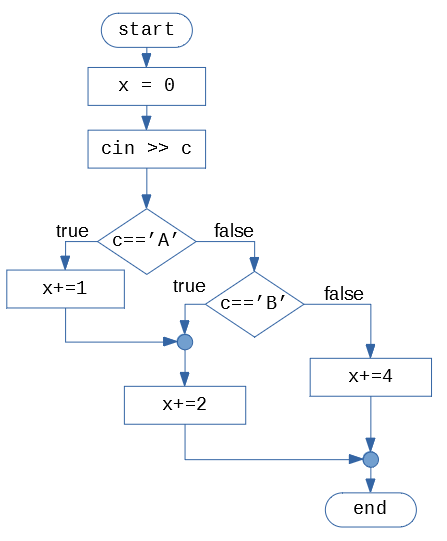
\includegraphics[width=3in]{assignment01-expr-control/assignment01-flowchart.png}

\vspace{20pt}
{\bf Question 3 (Side Effects).} Variable {\tt x} 
has value $3$ - initially it is $0$, but it is incremented by $1$, then by $2$
in two different case statements (notice, there is no {\tt break} after the 
first {\tt case}).

\end{document}



